\documentclass[12pt,a4paper,bibliography=totocnumbered,listof=totocnumbered]{article}
\usepackage[ngerman]{babel}
\usepackage[utf8]{inputenc}
%\titlespacing{\section}{0pt}{12pt plus 4pt minus 2pt}{-6pt plus 2pt minus 2pt}

% Kopf- und Fusszeile
\renewcommand{\sectionmark}[1]{\markright{#1}}
\renewcommand{\leftmark}{\rightmark}
\pagestyle{fancy}
\lhead{}
\chead{}
\rhead{\thesection\space\contentsname}
\lfoot{Implementierung von Brettspielen am Beispiel ReversiXT -- SS \the\year}
\cfoot{}
\rfoot{\ \linebreak Seite \thepage}
\renewcommand{\headrulewidth}{0.4pt}
\renewcommand{\footrulewidth}{0.4pt}

% Vorspann
\renewcommand{\thesection}{\Roman{section}}
\renewcommand{\theHsection}{\Roman{section}}
\pagenumbering{Roman}

\newcommand{\folgen}[1]{
\ensuremath
#1
}

\newcommand{\MyTitlepage}[5][\empty]{
\thispagestyle{empty}
\begin{center}
	
\includegraphics[scale=0.2]{pics/oth-logo.png}\\
	\vspace*{2cm}
	\Large
	\textbf{Fakultät}\\
	\textbf{Informatik und Mathematik}\\
	\vspace*{2cm}
	\Huge
	\textbf{Projektbericht}\\
	\vspace*{0.5cm}
	\large
	zum Wahlpflichtfach im SS \the\year\\
	\vspace*{1cm}
	\textbf{Implementierung von Brettspielen am Beispiel ReversiXT}\\
	\vspace*{1cm}
	\includegraphics[height=6cm]{#1}
	\vfill
	\normalsize
	%\newcolumntype{x}[1]{>{\raggedleft\arraybackslash\hspace{0pt}}p{#1}}
	\begin{tabular}{rl}%{6cm}p{7.5cm}}
	    \rule{0mm}{5ex}\textbf{Gruppe:} & #2 \\
		\rule{0mm}{5ex}\textbf{Autoren:} & \hspace*{-0.5em}\begin{tabular}[t]{r}#3\end{tabular} \\ 
		\rule{0mm}{5ex}\textbf{Leiter:} & Prof. Dr. rer. nat. Carsten Kern \\ 
		\rule{0mm}{5ex}\textbf{Abgabedatum:} & #4 \\ 
	\end{tabular} 
\end{center}
\pagebreak
}

\begin{document}

% ----------------------------------------------------------------------------------------------------------
% Titelseite
% ----------------------------------------------------------------------------------------------------------
\MyTitlepage[pics/gamefield02]{???}{
\texttt{stud1@st.oth-regensburg.de}\\
\texttt{stud2@st.oth-regensburg.de}\\
\texttt{stud3@st.oth-regensburg.de}}
{??.??.\the\year} % FIXME optional: Gruppenlogo als PNG, Pflichtfelder: Gruppe, Authoren durch "\\" getrennt und Abgabedatum eingeben

\setcounter{page}{1} 
% ----------------------------------------------------------------------------------------------------------
% Inhaltsverzeichnis
% ----------------------------------------------------------------------------------------------------------
\tableofcontents
\pagebreak


% ----------------------------------------------------------------------------------------------------------
% Inhalt
% ----------------------------------------------------------------------------------------------------------
% Abstände Überschrift
%\titlespacing{\section}{0pt}{12pt plus 4pt minus 2pt}{6pt plus 2pt minus 2pt}
%\titlespacing{\subsection}{0pt}{12pt plus 4pt minus 2pt}{4pt plus 2pt minus 2pt}
%\titlespacing{\subsubsection}{0pt}{12pt plus 4pt minus 2pt}{2pt plus 2pt minus 2pt}

% Kopfzeile
\renewcommand{\sectionmark}[1]{\markright{#1}}
\renewcommand{\subsectionmark}[1]{}
\renewcommand{\subsubsectionmark}[1]{}
\lhead{Kapitel \thesection}
\rhead{\rightmark}

\onehalfspacing
\renewcommand{\thesection}{\arabic{section}}
\renewcommand{\theHsection}{\arabic{section}}
\setcounter{section}{0}
\pagenumbering{arabic}
\setcounter{page}{1}

% ----------------------------------------------------------------------------------
% Kapitel: Einleitung
% ----------------------------------------------------------------------------------
\section{Einleitung}
Leiten Sie in diesem Abschnitt in das Wahlpflichtfach \emph{ZOCK} und das in diesem Zusammenhang zu erstellende Projekt ein.

Beschreiben Sie dazu das Spiel ReversiXT in einigen Sätzen (wie funktioniert das Grundspiel und welche Besonderheiten gibt es gegenüber dem üblichen Reversi). Fügen Sie evtl.\ auch einen Screenshot einer Spielkarte ein (mit dem im April bereitgestellten Spielfeld-Editor), der interessante Eigenschaften des Spiels widerspiegelt. Denken Sie immer daran, eingefügte Bilder sowohl aus dem Text heraus zu referenzieren als auch diese Bilder mit eigenen Worten zu erklären. Erläutern Sie dann ebenfalls die Fragestellung, die in diesem Wahlpflichtfach gelöst werden soll.

Beschreiben Sie in diesem Kapitel zusätzlich in einigen Sätzen, was Sie sich von diesem Wahlpflichtfach versprechen, um zu einem späteren Zeitpunkt im Fazit zu klären, welche persönlichen Erwartungen sich erfüllt haben und welche vielleicht offen geblieben sind.

Der Umfang dieses Abschnitts sollte bei finaler Abgabe mindestens eine DIN-A4-Seite betragen.

\bigskip

\textbf{Wichtige Hinweise zum gesamten Projektbericht:}
\begin{itemize}
  \item Achten Sie im ganzen Dokument auf korrekte Ausdrucksweise, Rechtschreibung, Zeichensetzung und Grammatik. Nutzen Sie für die Rechtschreibkorrektur einen Spellchecker (in \href{http://www.xm1math.net/texmaker/}{Texmaker} bereits integriert) und lassen Sie alle Abschnitte von allen Gruppenmitgliedern vor der Abgabe intensiv Korrektur lesen. Stellen Sie sich vor, dass das vorliegende Dokument für Sie eine Abschlussarbeit darstellt, die bei Abgabe eine sehr gute Form haben muss. Die Form der Arbeit und die Anzahl der darin enthaltenen Fehler wird - wie auch beim Praxisbericht im 5.\ Semester bzw.\ bei der Bachelorarbeit im 7.\ Semester - eine Auswirkung auf die Note des Projektberichts haben.
  \item Sobald Sie Bilder, Tabellen oder andere Arten von Abbildungen verwenden, so geben Sie ihnen eine Nummer samt Kurzbeschreibung und referenzieren Sie diese im Text. Ein Beispiel dafür finden Sie in Abschnitt \ref{Kap:Minipage} (damit die Referenz im PDF auch angezeigt wird, muss das Dokument u.\,U.\ zweimal kompiliert werden). Beschreiben Sie an der Stelle, an der die Abbildung referenziert wird auch immer deren Sinn/Inhalt/Bedeutung mit eigenen Worten. Eine Abbildung spricht niemals für sich selbst.
\end{itemize}

\newpage
% ----------------------------------------------------------------------------------
% Kapitel: Allgemeine Informationen
% ----------------------------------------------------------------------------------
\section{Allgemeine Informationen}
Versuchen Sie eine \emph{weiche} Überleitung in dieses Kapitel zu formulieren, indem Sie kurz beschreiben, was den Leser in diesem Kapitel erwartet und warum das interessant ist.
\subsection{Team und Kommunikation}
Beschreiben Sie in diesem Abschnitt ausführlich Ihr Team. Welche Personen aus welchen Studiengängen in welchem Semester bilden Ihr Team? Stellen Sie jeweils das vorhandene Vorwissen der Personen dar, das in dieser Veranstaltung für Sie von Nutzen sein könnte/ist/war, etc. Beschreiben Sie auch, wie/mit welchen Mitteln im Team regelmäßig kommuniziert wurde. Sollten Sie außerhalb der Vorlesungen und Übungen von ZOCK weitere regelmäßige Treffen vereinbart und abgehalten haben, so sollten Sie dies hier auch beschreiben.

Halten Sie außerdem in jeder Woche fest (z.\,B.\ in Form einer Tabelle), welche Person welche Aufgaben wahrgenommen hat, wie Aufgaben aufgeteilt wurden etc.

Der Umfang dieses Abschnitts sollte bei der ersten Deadline im April mindestens eine $\frac{1}{2}$-Seite betragen und am Ende inkl.\ der zu erstellenden Tabelle deutlich länger sein.

\subsection{Technische Daten}
Beschreiben Sie u.a.\ in welcher Programmiersprache (inkl.\ Version) und unter welchem Betriebssystem(en) (inkl.\ Version(en)) Sie entwickeln, welche IDEs (inkl. Versionen) Sie nutzen, welche zusätzlichen Tools bei Ihrer Projektentwicklung Einsatz gefunden haben und auf welcher Hardware Sie entwickelt und getestet haben etc.

Beschreiben Sie auch, warum Sie sich für diese Sprachen/Tools etc.\ entschieden haben (z.\,B.: welche Vorteile erhoffen Sie sich dadurch).

Der Umfang dieses Abschnitts sollte mindestens eine $\frac{1}{2}$-Seite betragen.

\subsection{Datenstruktur}
Beschreiben Sie detailliert die Datenstruktur, die Sie zur Speicherung des Spielfeldes in Ihrem Client nutzen. Gehen Sie auf Besonderheiten ein und erklären Sie, wie diese funktionieren und was Sie sich davon erhoffen. Gehen Sie auf die Vorteile (und evtl.\ Nachteile) ein, die Ihre Datenstruktur aus Ihrer Sicht hat. Geben Sie falls möglich auch eine schematische Darstellung/ein Bild der Datenstruktur an. Klären Sie insbesondere auch, wie Transitionen bei Ihnen repräsentiert werden. Auch hier könnte ein schematisches Bild beim Verständnis helfen.

Der Umfang dieses Abschnitts sollte mindestens eine $\frac{3}{4}$-Seite betragen.


\newpage
% ----------------------------------------------------------------------------------
% Kapitel: Spielfeldbewertung
% ----------------------------------------------------------------------------------
\section{Spielfeldbewertung}
Versuchen Sie eine \emph{weiche} Überleitung in dieses Kapitel zu formulieren, indem Sie kurz beschreiben, was den Leser in diesem Kapitel erwartet und warum das für die entstehende K.\,I.\ interessant ist.

\subsection{Bestandteile und Implementierung}\label{kap:Heuristik}
Beschreiben Sie detailliert, welche Elemente Sie in Ihrer Heuristik für Ihren Client umgesetzt. Beschreiben Sie dazu auch Werte von Parametern (Kriterien und Gewichtungen), die Sie in den einzelnen Implementierungen nutzen. Welche statischen Vorberechnungen Sie machen, um z.\,B.\ das Spielfeld zu analysieren, etc.

Nutzen Sie zum besseren Verständnis - wie auch in den vorhergehenden beiden Abschnitten - Bilder und erklären Sie jeweils, was darauf zu sehen ist.

Bei der finalen Abgabe des Dokuments im Juni ist dieser Abschnitt eines der wichtigsten Kapitel im gesamten Projektbericht. Stellen Sie sicher, dass am Ende alle Elemente der Heuristik, die Sie in Ihrem Client umgesetzt haben, auch in diesem Kapitel detailliert inkl.\ verwendeter Gewichtungen und Parameter etc.\ beschrieben werden.

Auch hier wäre eine Gegenüberstellung von Vor- und Nachteilen der einzelnen Heuristikbestandteile wünschenswert.

Der Umfang dieses Abschnitts sollte bei der ersten Abgabe im April mindestens eine $\frac{1}{2}$-Seite und bei der finalen Abgabe im Juni mindestens 2 Seiten betragen.

\newpage
% ----------------------------------------------------------------------------------
% Kapitel: Fazit
% ----------------------------------------------------------------------------------
\section{Fazit}
Beschreiben Sie in diesem Abschnitt u.a.\ was Ihnen an diesem Fach gefallen hat und welche Verbesserungsvorschläge Sie für künftige Veranstaltungen haben. Was konnten Sie dazulernen, in welchen Bereichen haben Sie sich verbessert. Welche Problemsituationen gab es während der Projekterstellung, wie sind Sie diese angegangen und wie haben Sie diese gelöst. Was haben Sie evtl.\ vermisst.


\newpage
% ----------------------------------------------------------------------------------
% Kleine Einführung in LaTeX-Elemente
% ----------------------------------------------------------------------------------
\section{\LaTeX-Elemente}
Dieser Abschnitt soll nicht Bestandteil des Projektberichtes sein, sondern beinhaltet lediglich einige Informationen über \LaTeX-Distributionen, Editoren und \LaTeX-Elemente, die Ihnen beim Einstieg in das \LaTeX-Textsatzsystem helfen sollen.

\subsection{\LaTeX-Distributionen nach Betriebssystemen}

\subsubsection{\LaTeX-Distributionen}
Folgende Haupt-\LaTeX-Distributionen stehen Ihnen zur Verfügung:
\begin{itemize}
  \item Windows:\quad \texttt{MiKTeX}\quad Webseite:\quad\url{http://www.miktex.org}
  \item Linux/Unix:\quad \texttt{TeX Live}\quad Webseite:\quad\url{http://tug.org/texlive/}
  \item Mac OS:\quad \texttt{MacTeX}\quad Webseite:\quad\url{http://www.tug.org/mactex/}
\end{itemize}

\subsubsection{\LaTeX-Editoren}
Auf folgenden Webseiten können Sie einige hilfreiche \LaTeX-Editoren finden:
\begin{itemize}
  \item Windows/Linux/Mac OS: \url{http://www.xm1math.net/texmaker/}
  \item Windiws: \url{http://www.texniccenter.org/}
  \item Mac OS: \url{http://pages.uoregon.edu/koch/texshop/}
\end{itemize}

Falls bei den oben genannten Editoren kein passender vorhanden war, findet sich auf Wikipedia eine Zusammenstellung vieler weiterer \LaTeX-Editoren:\\[1em]
\hspace*{3cm}\url{https://en.wikipedia.org/wiki/Comparison_of_TeX_editors}


\subsection{Unterabschnitt}\label{Kap:Minipage}
Zum Einfügen eines Bildes, siehe Abbildung \ref{fig:reversi01}, wird die \textit{minipage}-Umgebung genutzt, da die Bilder so gut positioniert werden können.

\vspace{1em}
\begin{minipage}{\linewidth}
	\centering
	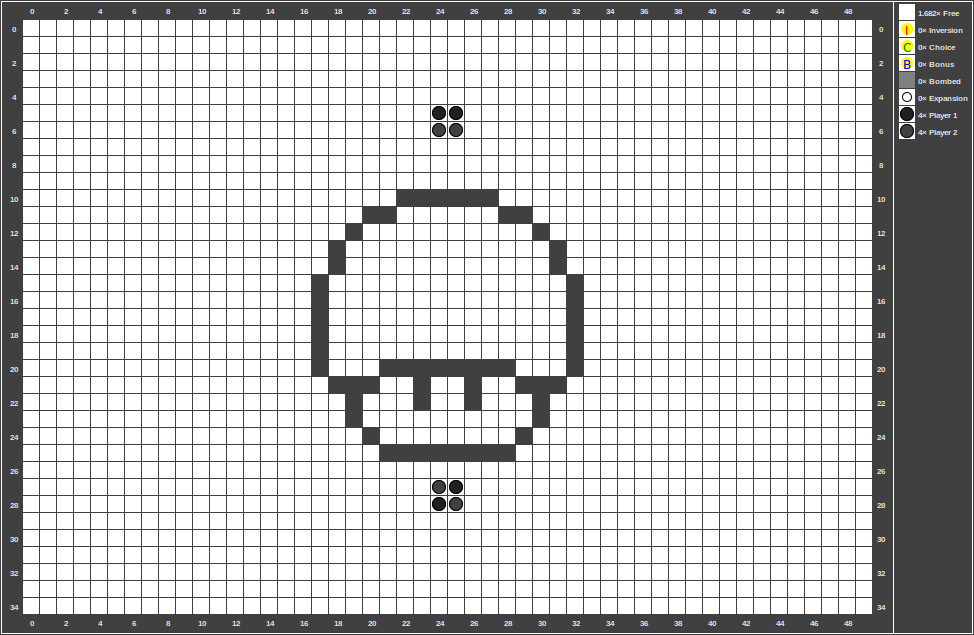
\includegraphics[width=0.6\linewidth]{pics/gamefield01.png}
	\captionof{figure}[Spielfeld 01]{Unbespieltes Spielfeld\footnotemark }
	\label{fig:reversi01}
\end{minipage}
\footnotetext{Diesem Spielfeld wurden noch keine Spieler zugewiesen (daher die dunklen Spielsteine)}

Nachdem das Spielt gestartet wurde und beide Spielphasen durchlaufen wurden, siegt schließlich der Spieler mit der Farbe rot.

\vspace{1em}
\begin{minipage}{\linewidth}
	\centering
	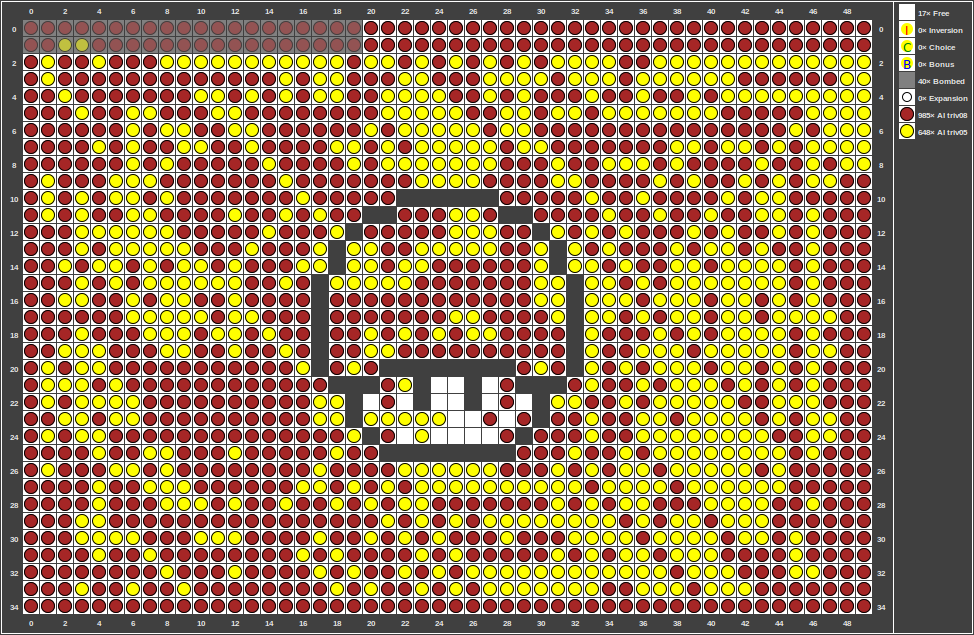
\includegraphics[width=0.6\linewidth]{pics/gamefield02.png}
	\captionof{figure}[Spielfeld 02]{Finales Spielfeld\footnotemark }
	\label{fig:reversi2}
\end{minipage}
\footnotetext{Das Spielfeld nach der Zug- und Bombenphase. Spieler rot gewinnt eindeutig.}

\subsection{Tabellen}
In diesem Abschnitt wird eine Tabelle (siehe Tabelle \ref{tab:beispiel}) dargestellt.

\vspace{1em}
\begin{table}[!h]
	\centering
	\begin{tabular}{|l|l|l|}
		\hline
		\textbf{Name} & \textbf{Name} & \textbf{Name}\\
		\hline
		1 & 2 & 3\\
		\hline
		4 & 5 & 6\\
		\hline
		7 & 8 & 9\\
		\hline
	\end{tabular}
	\caption{Beispieltabelle}
	\label{tab:beispiel}
\end{table}


\subsection{Auflistung}
Für Auflistungen wird die \texttt{enumerate}- oder \texttt{itemize}-Umgebung genutzt.

\begin{itemize}
	\item Nur
	\item ein
	\item Beispiel.
\end{itemize}

\subsection{Listings}
\subsection{Listings}
Zuletzt sehen Sie in Listing \ref{lst:maxTeilsumZweiD} ein Beispiel für das Einbinden von Quellcode mit Syntax-Highlighting.

\vspace{1em}
\lstinputlisting[caption=Brute Force-Ansatz für das MaxTeilsum2D-Problem, label=lst:maxTeilsumZweiD,basicstyle=\ttfamily\scriptsize]{code/maxTeilsum2DBruteForce.txt}

\subsection{Selbstgestaltete Abbildungen}
Mithilfe des Paketes \texttt{tikz} können sehr schöne Abbildungen (z.\,B.\ Automaten, Graphen etc.) direkt in \LaTeX generiert werden. Viele Beispiele dazu finden Sie auf folgender Webseite:\\[1em]
\hspace*{3cm}\url{http://www.texample.net/tikz/}.

\subsection{Tipps}
Die Quellen befinden sich in der Datei \textit{quellen.bib}. Eine Buch- und eine Online-Quelle sind beispielhaft eingefügt. [Vgl. \cite{buch}, \cite{online}]

\pagebreak

% ----------------------------------------------------------------------------------------------------------
% Kapitel
% ----------------------------------------------------------------------------------------------------------
\section{Kapitel}
Lorem ipsum dolor sit amet.

\subsection{Unterkapitel}
Lorem ipsum dolor sit amet, consetetur sadipscing elitr, sed diam nonumy eirmod tempor invidunt ut labore et dolore magna aliquyam erat, sed diam voluptua. At vero eos et accusam et justo duo dolores et ea rebum. Stet clita kasd gubergren, no sea takimata sanctus est Lorem ipsum dolor sit amet. Lorem ipsum dolor sit amet, consetetur sadipscing elitr, sed diam nonumy eirmod tempor invidunt ut labore et dolore magna aliquyam erat, sed diam voluptua. At vero eos et accusam et justo duo dolores et ea rebum. Stet clita kasd gubergren, no sea takimata sanctus est Lorem ipsum dolor sit amet.

\subsection{Unterkapitel}
Lorem ipsum dolor sit amet, consetetur sadipscing elitr, sed diam nonumy eirmod tempor invidunt ut labore et dolore magna aliquyam erat, sed diam voluptua. At vero eos et accusam et justo duo dolores et ea rebum. Stet clita kasd gubergren, no sea takimata sanctus est Lorem ipsum dolor sit amet. Lorem ipsum dolor sit amet, consetetur sadipscing elitr, sed diam nonumy eirmod tempor invidunt ut labore et dolore magna aliquyam erat, sed diam voluptua. At vero eos et accusam et justo duo dolores et ea rebum. Stet clita kasd gubergren, no sea takimata sanctus est Lorem ipsum dolor sit amet.
\pagebreak

% ----------------------------------------------------------------------------------------------------------
% Literatur
% ----------------------------------------------------------------------------------------------------------
\renewcommand\refname{Quellenverzeichnis}
\bibliographystyle{alpha}
\bibliography{quellen}
\pagebreak

% ----------------------------------------------------------------------------------------------------------
% Anhang
% ----------------------------------------------------------------------------------------------------------
\pagenumbering{Roman}
\setcounter{page}{1}
\lhead{Anhang \thesection}

\begin{appendix}
\section*{Anhang}
\phantomsection
\addcontentsline{toc}{section}{Anhang}
\addtocontents{toc}{\vspace{-0.5em}}

\section{GUI}
Ein toller Anhang.

\subsection*{Screenshot}
\label{app:screenshot}
Unterkategorie, die nicht im Inhaltsverzeichnis auftaucht.

\end{appendix}


\end{document}
